\begin{frontmatter}

    \title{Dam Site Selection for Expansion in Morocco using Multi-Criteria Decision-Making}

    \author[opj]{John Oppong\corref{mycorrespondingauthor}}
    \ead{john.oppong@um6p.ma}
    \author[abs-supervisor]{Prof. Noureddine Kouaissah}
    \ead{Noureddine.KOUAISSAH@um6p.ma}
    \author[sci-supervisor]{Prof. Edmond Seabright}
    \ead{Edmond.Seabright@um6p.ma}

    \affiliation[UM6P]{organization={Mohammed VI Polytechnic University},
             addressline={Lot 660, Hay Moulay Rachid},
             city={Benguerir},
             postcode={3000},
             state={BG},
             country={Morocco}}


\begin{abstract}
Water scarcity poses a critical challenge to Morocco, where dams remain central to national strategies for irrigation, hydropower, and water supply. Selecting suitable sites for dam expansion is a complex decision problem, requiring the balance of technical, economic, social, and environmental objectives. This study applies Multi-Criteria Decision-Making (MCDM) through four Goal Programming (GP) variants—Weighted (WGP), Lexicographic (LGP), Chebyshev (CGP), and Extended (EGP)—to the selection of three dams from twenty-eight candidates under a fixed budget constraint. To reflect policy uncertainty, Multi-Choice Goal Programming (MCGP) extensions were incorporated for key socio-environmental targets (population, farmland area, residence distance, farmland distance, and road access). Results identify dams 18, 19, and 20 as a consistently robust core across models and scenarios, while dams 28, 21, and 23 emerge as flexible alternatives when environmental or social criteria are emphasized. Sensitivity analysis on both weights and targets confirms that WGP and LGP provide stable recommendations, whereas CGP and EGP display greater variability. These findings suggest that GP does not yield a single rigid solution but rather a decision space that combines stability with adaptability, allowing policymakers to reconcile competing objectives. Beyond the case of Morocco, the study contributes methodologically by integrating multi-choice goals and systematic sensitivity analysis into GP, and theoretically by framing dam site selection as a problem of compromise and robustness rather than strict optimization. The approach offers a transparent, adaptable, and policy-relevant decision-support tool for sustainable water infrastructure planning under uncertainty.
\end{abstract}


    \begin{graphicalabstract}
        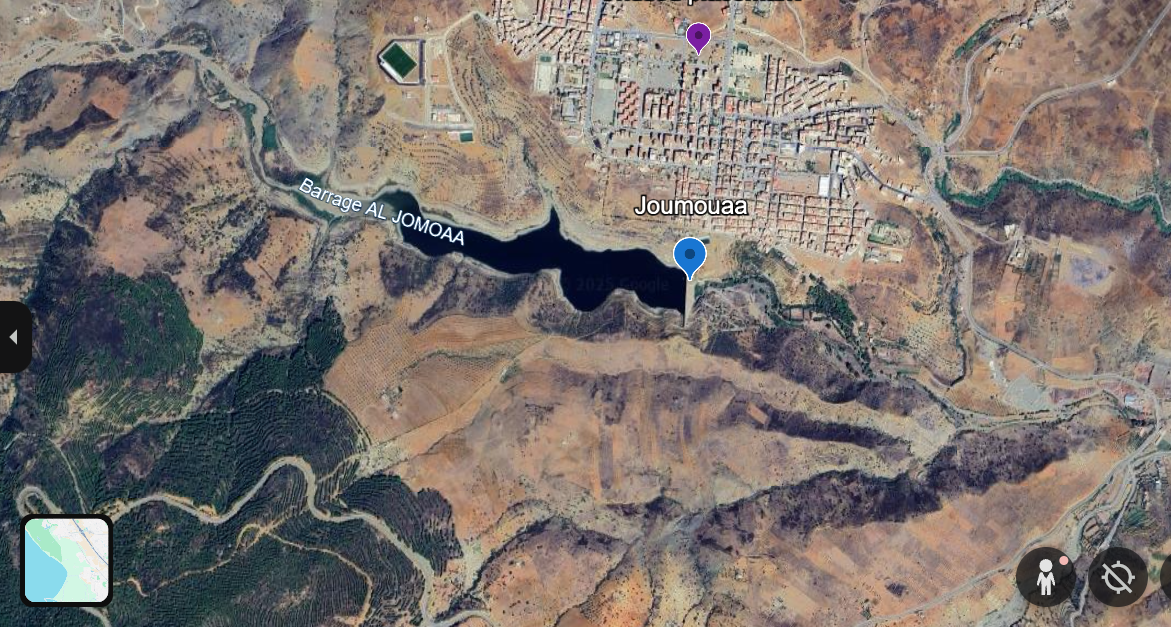
\includegraphics[width=\linewidth]{figures/joumaa}
    \end{graphicalabstract}

    % Research highlights
    \begin{highlights}
        \item Dam sites 18, 19, 20, and 28 appear most often in the results, making them reliable choices for Morocco's urgent dam site expansion needs.
        \item The four GP models (\gls{WGP}, \gls{LGP}, \gls{CGP}, \gls{EGP}) were extended with Multi-Choice Goal Programming to reflect the reality of multiple targets and choices in decision-making.
        \item Goal programming was adopted for its closeness in underlying principles with Collective Intelligence.
    \end{highlights}

    \begin{keyword}
        Multi-Criteria Decision-Making \sep Goal Programming \sep Dam Site Selection \sep Water Resource Management \sep Morocco
    \end{keyword}

\end{frontmatter}   
